\documentclass[
  bibliography=totoc,     % Literatur im Inhaltsverzeichnis
  captions=tableheading,  % Tabellenüberschriften
  titlepage=firstiscover, % Titelseite ist Deckblatt
]{scrartcl}

% Paket float verbessern
\usepackage{scrhack}

% Warnung, falls nochmal kompiliert werden muss
\usepackage[aux]{rerunfilecheck}

% unverzichtbare Mathe-Befehle
\usepackage{amsmath}
% viele Mathe-Symbole
\usepackage{amssymb}
% Erweiterungen für amsmath
\usepackage{mathtools}

% Fonteinstellungen
\usepackage{fontspec}
% Latin Modern Fonts werden automatisch geladen
% Alternativ:
%\setromanfont{Libertinus Serif}
%\setsansfont{Libertinus Sans}
%\setmonofont{Libertinus Mono}
\recalctypearea % Wenn man andere Schriftarten gesetzt hat,
% sollte man das Seiten-Layout neu berechnen lassen

% deutsche Spracheinstellungen
\usepackage{polyglossia}
\setmainlanguage{german}


\usepackage[
  math-style=ISO,    % ┐
  bold-style=ISO,    % │
  sans-style=italic, % │ ISO-Standard folgen
  nabla=upright,     % │
  partial=upright,   % ┘
  warnings-off={           % ┐
    mathtools-colon,       % │ unnötige Warnungen ausschalten
    mathtools-overbracket, % │
},                       % ┘
]{unicode-math}

% traditionelle Fonts für Mathematik
\setmathfont{Latin Modern Math}
% Alternativ:
%\setmathfont{Libertinus Math}

\setmathfont{XITS Math}[range={scr, bfscr}]
\setmathfont{XITS Math}[range={cal, bfcal}, StylisticSet=1]

% Zahlen und Einheiten
\usepackage[
locale=DE,                   % deutsche Einstellungen
separate-uncertainty=true,   % immer Fehler mit \pm
per-mode=symbol-or-fraction, % / in inline math, fraction in display math
]{siunitx}

% chemische Formeln
\usepackage[
version=4,
math-greek=default, % ┐ mit unicode-math zusammenarbeiten
text-greek=default, % ┘
]{mhchem}

% richtige Anführungszeichen
\usepackage[autostyle]{csquotes}

% schöne Brüche im Text
\usepackage{xfrac}

% Standardplatzierung für Floats einstellen
\usepackage{float}
\floatplacement{figure}{htbp}
\floatplacement{table}{htbp}

% Floats innerhalb einer Section halten
\usepackage[
section, % Floats innerhalb der Section halten
below,   % unterhalb der Section aber auf der selben Seite ist ok
]{placeins}

% Seite drehen für breite Tabellen: landscape Umgebung
\usepackage{pdflscape}

% Captions schöner machen.
\usepackage[
  labelfont=bf,        % Tabelle x: Abbildung y: ist jetzt fett
  font=small,          % Schrift etwas kleiner als Dokument
  width=0.9\textwidth, % maximale Breite einer Caption schmaler
]{caption}
% subfigure, subtable, subref
\usepackage{subcaption}

% Grafiken können eingebunden werden
\usepackage{graphicx}
% größere Variation von Dateinamen möglich
\usepackage{grffile}

% schöne Tabellen
\usepackage{booktabs}

% Verbesserungen am Schriftbild
\usepackage{microtype}

% Literaturverzeichnis
\usepackage[style=alphabetic,]{biblatex}
% Quellendatenbank
\addbibresource{lit.bib}

% Hyperlinks im Dokument
\usepackage[
  unicode,        % Unicode in PDF-Attributen erlauben
  pdfusetitle,    % Titel, Autoren und Datum als PDF-Attribute
  pdfcreator={},  % ┐ PDF-Attribute säubern
  pdfproducer={}, % ┘
]{hyperref}
% erweiterte Bookmarks im PDF
\usepackage{bookmark}

% Trennung von Wörtern mit Strichen
\usepackage[shortcuts]{extdash}

\title{V351: Fourier-Analyse und Synthese}
\author{
  Simon Schulte
  \texorpdfstring{
    \\
    \href{mailto:simon.schulte@udo.edu}{simon.schulte@udo.edu}
  }{}
  \texorpdfstring{\and}{, }
  Tim Sedlaczek
  \texorpdfstring{
    \\
    \href{mailto:tim.sedlaczek@udo.edu}{tim.sedlaczek@udo.edu}
  }{}
}
\publishers{TU Dortmund – Fakultät Physik}

\date{Durchführung: 17.1.2017\\
      Abgabe: 24.01.2016}


\begin{document}

\maketitle
\thispagestyle{empty}
\tableofcontents
\newpage
\section{Zielsetzung}
\label{sec:zielsetzung}
Ziel des Versuchs ist es, mit Hilfe der Fourier-Analyse eine zeitlich periodische
Spannungsschwingung in ihre einzelnen Fourier-Komponenten zu zerlegen, sowie
eine solche Schwingung aus ihren Komponenten zu synthetisieren.
\section{Theorie}
\label{sec:theorie}
Schwingungen sind räumlich oder zeitlich wiederkehrende periodische Veränderungen.
Sie treten also entweder nach einer bestimmten Periodendauer oder einer
bestimmten Entfernung wieder auf. Schwingungen lassen sich theoretisch immer
als sinus- oder cosinusfunktion beschreiben. \\
\\
Das Fouriersche Theorem versucht jede Schwingung aus einer Kombination von
sinus- und cosinusfunktionen zu charakterisieren. So lässt sich eine periodische
Funktion $f(t)$ mit der Periodendauer $T$ darstellen als:
\begin{equation}
	\frac{1}{2}a_0+\sum_{n=1}^{\infty}\left(a_n\cos\left(n\frac{2\pi}{T}t\right)+b_n\sin\left(n\frac{2\pi}{T}t\right)\right),\:\:\:n\in\mathbb{N}
	\label{eqn:fourier_theorem}
\end{equation}
$a_n$ und $b_n$ sind die Fourier-Koeffizienten. Diese lassen sich mit diesen
Gleichungen bestimmen:
\begin{align}
	a_n=&\frac{2}{T}\int_0^T f(t)\cos\left(n\frac{2\pi}{T}t\right)\mathup{d}t&\\
	b_n=&\frac{2}{T}\int_0^T f(t)\sin\left(n\frac{2\pi}{T}t\right)\mathup{d}t&n=1,2,\ldots
	\label{eqn:fourier_koeffizienten}
\end{align}
Gleichung \eqref{eqn:fourier_theorem} gilt nur, falls $f(t)$ stetig ist und die
unendliche Potenzreihe gleichmäßig konvergiert. Wenn $f$ an einer Stelle nicht
stetig ist, treten Abweichungen in der Approximation durch die Fourier-Reihe
auf, sofern diese nur bis zu einer endlich hohen Oberwelle betrachtet wird.
Dieser Effekt wird Gibbsches Phänomen genannt.
\subsection{Fourier-Transformation}
Neben der Darstellung als Fourier-Reihe und einer Zerlegung in $n$ Schwingungen,
ist es auch möglich aus einer Funktion $f(t)$ das Frequenzspektrum zu bestimmen.
Dies wird dann als Fourier-Transformation bezeichnet. Es ist bei der Fourier-Transformation
nicht von Bedeutung, ob $f(t)$ eine periodische Funktion ist. Außerdem ist die
Fourier-Transformation umkehrbar. Es gilt:
\begin{equation}
	g(\nu)=\int_{-\infty}^{\infty}f(t)\mathup{e}^{\mathup{i}\nu t}\mathup{d}t.
	\label{eqn:fourier_trafo}
\end{equation}
Dabei ist $g(\nu)$ das Frequenzspektrum der Funktion $f(t)$. Sollte es sich bei
$f(t)$ um eine periodische Funktion handeln, besteht das Frequenzspektrum aus
Delta-Funktionen. Damit ist es dann ein diskretes Spektrum. Wenn $f(t)$ nicht
periodisch ist handelt es sich um ein kontinuierliches Spektrum. Das im Versuch
verwendete Oszilloskop ist in der Lage eine Fouriertransformation mit diskreten
Daten automatisch durchzuführen. Dabei muss das Abtasttheorem beachtet werden,
welches besagt, dass die Abtastfrequenz eines Messgerätes mindestens zweimal so
groß, wie die größte zu untersuchende Frequenz einer Oberwelle sein sollte. Wird
also bis zur $n$-ten Oberwelle untersucht, so gilt
\begin{equation}
	\nu_{\mathup{A}}>2n\nu_1,
	\label{eqn:abtasttheorem}
\end{equation}
wobei $\nu_{\mathup{A}}$ die Abtastfrequenz und $\nu_1$ die Frequenz der
Grundschwingung ist.
\subsection{Die Rechteck-, Dreieck- und Sägezahnspannung}
\label{sub:formeln}
Es werden in dem Versuch drei verschiedene Spannungsverläufe untersucht.
Die erste untersuchte Spannung, die Rechteckspannung, wird zur Vereinfachung
als ungerade Funktion definiert. Daher gilt:
\begin{equation}
	a_n=0
\end{equation}
Es ergibt sich desweiteren:
\begin{equation}
	b_n=
	\begin{cases}
		0,  & n \:\:\mathup{gerade}\\
		\frac{4}{n\pi}, &n \:\:\mathup{ungerade}
	\end{cases}
  \label{eqn:rechteck}
\end{equation}
Auch die zweite untersuchte Spannung, die Sägezahnspannung, wird als ungerade
Funktion definiert. Folglich gilt auch hier:
\begin{equation}
	a_n=0
\end{equation}
Desweiteren ergibt die Rechnung für den Koeffizienten der zweiten Summe:
\begin{equation}
	b_n=\left( -1 \right)^{n+1} \cdot \frac{2}{n}
  \label{eqn:sägezahn}
\end{equation}
Die dritte untersuchte Spannung, die Dreieckspannung, wird zur Vereinfachung
als gerade Funktion definiert. Es folgt:
\begin{equation}
	b_n=0
\end{equation}
Für $a_n$ gilt:
\begin{equation}
	a_n=
	\begin{cases}
		0,  & n \:\:\mathup{gerade}\\
		-\frac{4}{n^2\pi}, &n \:\:\mathup{ungerade}
	\end{cases}
  \label{eqn:dreieck}
\end{equation}
\clearpage
\section{Durchführung}
\subsection{Die Fourier-Analyse}
\begin{figure}[htb]
  \centering
  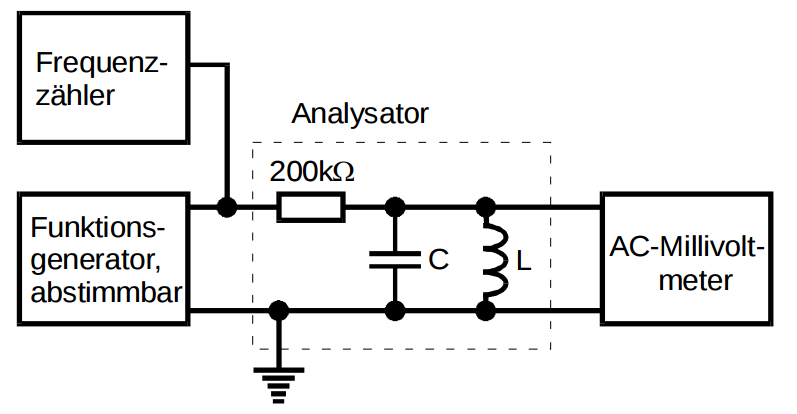
\includegraphics[width=0.75\textwidth]{V3511.png}
  \caption{Schematische Darstellung der Fourier-Analyse mit einem Speicheroszilloskop \cite{anleitung}.}
  \label{fig:V3511}
\end{figure}
In Abbildung \ref{fig:V3511} ist ein regelbarer Funktionsgenerator, der mit einem
digitalen Speicheroszilloskop verbunden ist, zu sehen. Es werden zunächst drei
verschiedene periodische Spannungsverläufe in ihre Oberwellen zerlegt.
Durch das Einstellen des Math-Modus im Oszilloskop werden die Spannungsverläufe
in ihre einzelnen Frequenzen zerlegt. Dadurch können die Amplituden der
einzelnen Bestandteile abgelesen werden. Es wird am Frequenzgenerator eine
Rechteck-, eine Dreieck- und eine Sägezahnspannung erzeugt. Das Frequenzspektrum
der jeweiligen Spannung wird mit Hilfe des Oszilloskops gebildet. Am
Oszilloskop können dann die einzelnen Peaks abgelesen werden und so für die
verschiedenen Oberwellen die Amplituden aufgenommen werden. Diese Werte
sollten dann, abhängig von der Höhe der Grundschwingung, mit den berechneten
Werten übereinstimmen.
\subsection{Die Fourier-Synthese}
Zur Synthese einer zeitlich periodischen Stromschwingung werden zu den
Frequenzen der Oberwellen jeweils die einzelnen Amplituden benötigt. Dafür werden
die Formeln aus \ref{sub:formeln} genutzt. Mit den Koeffizienten lässt sich das
Verhältniss der $n$-ten zur $n-1$-ten Oberwelle bestimmen und so, in Abhängigkeit
der Amplitude der ersten Oberwelle, die Amplitude der einzelnen Oberwellen bestimmen.
Dabei ist zu beachten, dass sowohl bei der Rechteck- als auch bei der Dreieckspannung
die geraden Koeffizienten keine Amplitude besitzen sollen, weshalb das Verhältniss, der
ungeraden Koeffizienten zueinander zu bestimmen ist.
Sind Frequenz und Amplitude der benötigten Oberwelle bekannt, lässt sich die Schwingung
mit Hilfe eines Oberwellengenerators synthetisieren. Dabei werden die ersten 10 Oberwellen am
Generator eingestellt und so in Phase gebracht, dass das Ergebnis der zu
erzeugenden Spannung möglichst nahe kommt.
\newpage
\section{Auswertung}
\label{sec:auswertung}
\subsection{Messwerte}
Mit dem Osziloskop wurden die in den Tabellen \ref{tab:messwerte1} und \ref{tab:messwerte2}
stehenden Werte für die Amplituden und Frequenzdifferenzen, der Oberschwingungen, gemessen.
\begin{table}
  \centering
  \caption{Messwerte zur Sägezahnspannung.}
  \label{tab:messwerte1}
  \sisetup{table-format=2.1}
  \begin{tabular}{S[table-format=1.0] S S[table-format=1.2] S[table-format=1.3]}
    \toprule
    {n} & {$\Delta f \,/\, \si{\kilo\hertz}$} & {$U \,/\, \si{\volt}$} & {$\frac{U}{U_0}$}\\
    \midrule
    1 & 10.5 & 4.44 & 1.000\\
    2 & 20.5 & 2.24 & 0.505\\
    3 & 30.5 & 1.5 & 0.338\\
    4 & 40.5 & 1.12 & 0.252\\
    5 & 50.5 & 0.88 & 0.198\\
    6 & 60.5 & 0.74 & 0.167\\
    7 & 70.5 & 0.64 & 0.144\\
    8 & 80.5 & 0.56 & 0.126\\
    9 & 90.5 & 0.5 & 0.113\\
    \bottomrule
  \end{tabular}
\end{table}
\begin{table}
  \centering
  \caption{Messwerte zur Rechteck- und Dreieckspannung.}
  \label{tab:messwerte2}
  \sisetup{table-format=1.3}
  \begin{tabular}{S[table-format=1.0] S[table-format=2.1] S[table-format=1.2] S S[table-format=1.4] S}
    \toprule
    & & \multicolumn{2}{c}{Rechteck} & \multicolumn{2}{c}{Dreieck}\\
    {n} & {$\Delta f \,/\, \si{\kilo\hertz}$} & {$U \,/\, \si{\volt}$} & {$\frac{U}{U_0}$} & {$U \,/\, \si{\volt}$} & {$\frac{U}{U_0}$}\\
    \midrule
    1 & 10.5 & 8.88 & 1.000 & 5.6 & 1.000\\
    3 & 20.5 & 2.88 & 0.324 & 0.62 & 0.111\\
    5 & 30.5 & 1.68 & 0.189 & 0.214 & 0.038\\
    7 & 40.5 & 1.14 & 0.128 & 0.0888 & 0.016\\
    9 & 50.5 & 0.82 & 0.092 & 0.048 & 0.009\\
    11 & 60.5 & 0.62 & 0.070 & 0.034 & 0.006\\
    \bottomrule
  \end{tabular}
\end{table}
\clearpage
\subsection{Fourier-Transformation(Analyse)}
Zur bestimmung der $n$-Abhängigkeiten wird zunächst der Logarithmus von $\frac{U}{U_0}$
gegen den Logarithmus von $n$ aufgetragen und mit einer linearen Funktion
\begin{equation}
  y = m \cdot x + b
\end{equation}
gefittet. Hierzu wird Python
verwendet. Die Steigung der Geraden gibt dann die exponentielle Abhängigkeit, der Koeffizienten,
von $n$ an.\\
Mit den in Tabelle \ref{tab:messwerte1} stehenden Werten ergibt sich, für die Sägezahnspannung
eine Steigung von $m = \num{-0.998(4)}$. Somit nehmen die Koeffizienten mit $\frac{1}{n}$ ab.
Der Verlauf der Messwerte und der Funktion sind in Abbildung \ref{fig:plot1} zu sehen.
\begin{figure}
  \centering
  \includegraphics[width=\textwidth]{Sägezahn.pdf}
  \caption{Logarithmus der Spannungsamplitude in Abhängigkeit von dem Logarithmus von $n$ (Sägezahn).}
  \label{fig:plot1}
\end{figure}
\clearpage
Als Steigung der Ausgleichsgeraden, der Rechteckspannung, ergibt sich, mit den Werten aus
Tabelle \ref{tab:messwerte2}, $m = \num{-1.10(3)}$. Die Koeffizienten nehmen demnach
mit $\frac{1}{n^{1.1}}$ ab. Im Idealfall wäre es eine $\frac{1}{n}$ Abhängigkeit, wie
an dem in \ref{sub:formeln} bestimmten Koeffizienten zu sehen ist.
Die entsprechende Kurve ist in Abbildung \ref{fig:plot2} zu sehen.
\begin{figure}
  \centering
  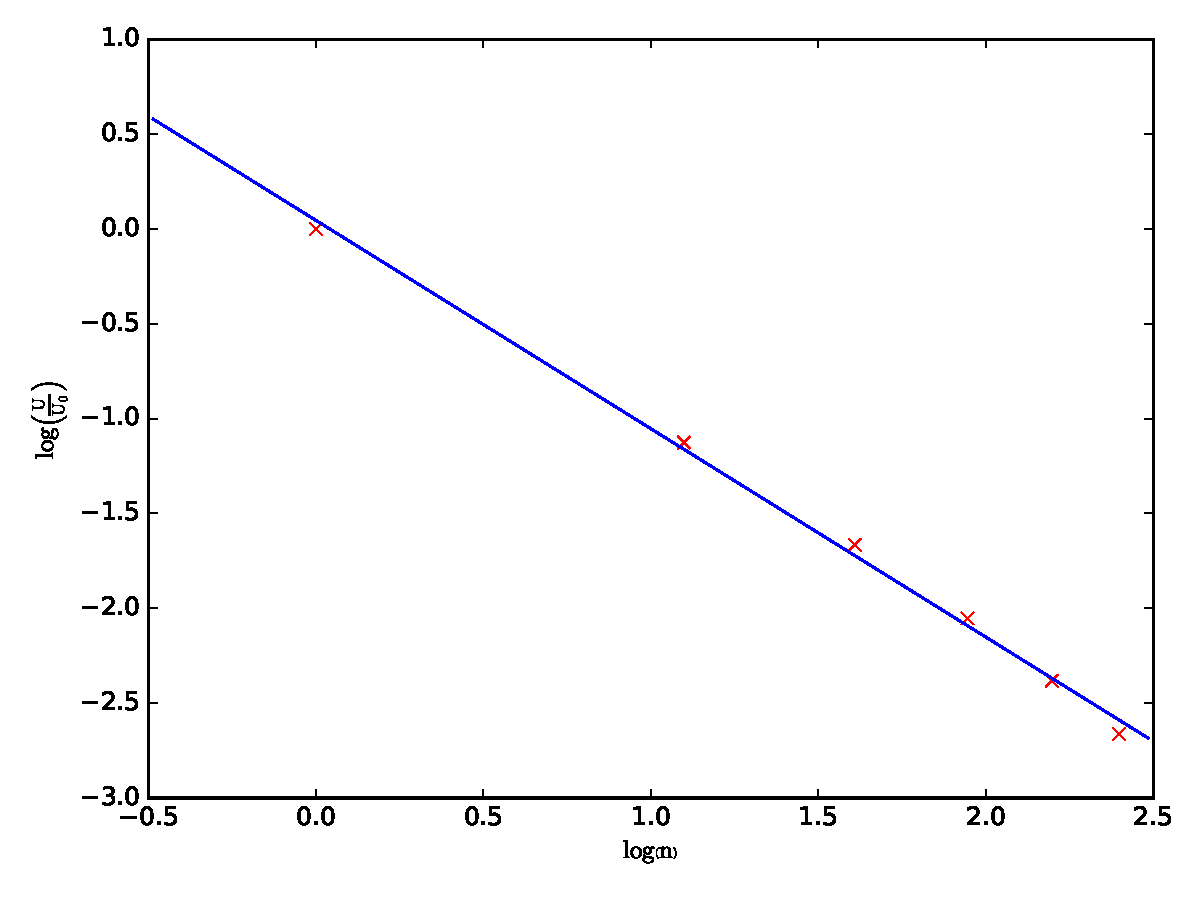
\includegraphics[width=\textwidth]{Rechteck.pdf}
  \caption{Logarithmus der Spannungsamplitude in Abhängigkeit von dem Logarithmus von $n$ (Rechteck).}
  \label{fig:plot2}
\end{figure}
\clearpage
Für die Dreieckspannung ergibt sich eine Steigung von $m = \num{-2.16(5)}$. Daraus
folgt eine $\frac{1}{n^{2.16}}$ Abhängigkeit. Der Optimalfall wäre eine Abnahme
nach $\frac{1}{n^2}$ gewesen. Der Graph ist in Abbildung \ref{fig:plot3} zu sehen.
\begin{figure}
  \centering
  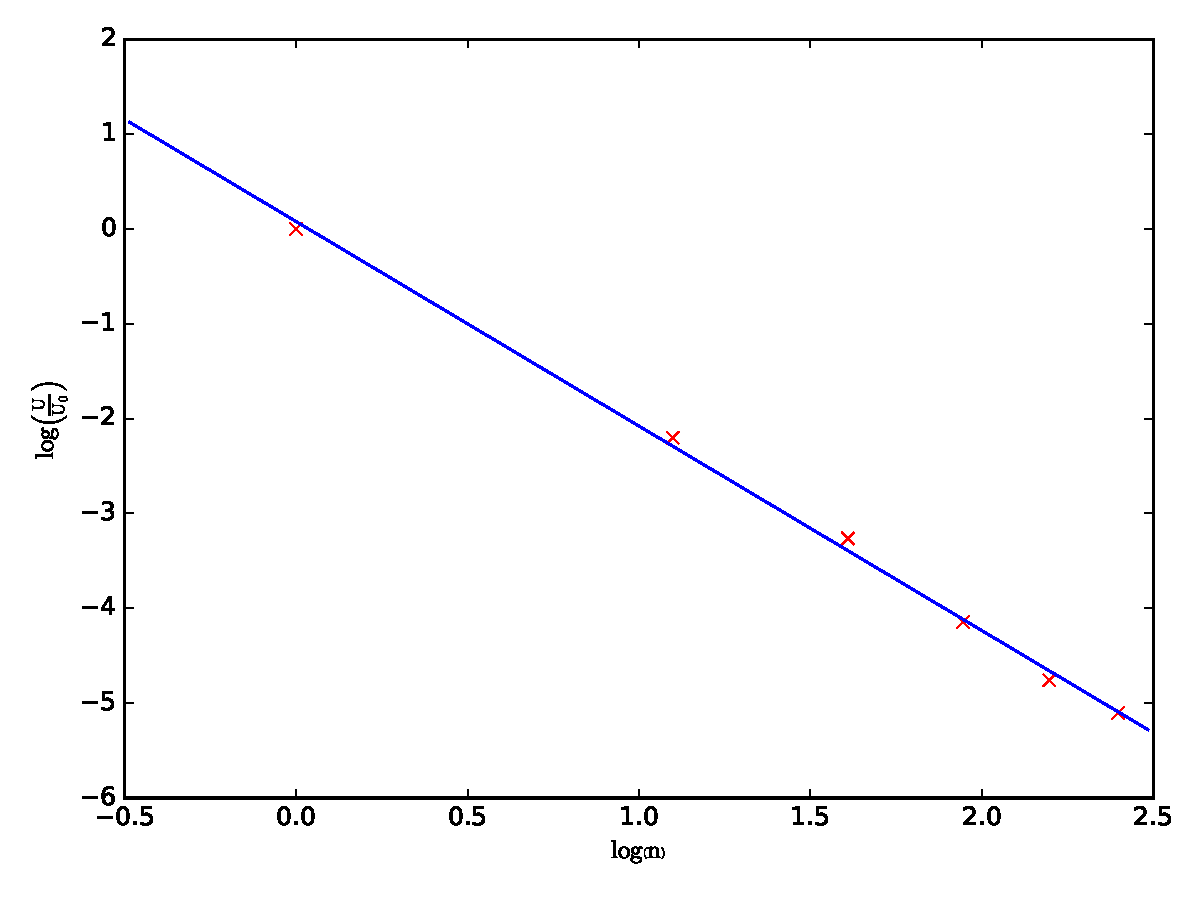
\includegraphics[width=\textwidth]{Dreieck.pdf}
  \caption{Logarithmus der Spannungsamplitude in Abhängigkeit von dem Logarithmus von $n$ (Dreieck).}
  \label{fig:plot3}
\end{figure}
\clearpage
\subsection{Fourier-Synthese}
Für die Synthese werden zunächst die Verhältnisse der Amplituden bestimmt und danach
die Amplitunden der Oberwellen entsprechend eingestellt. Die Ausgangsamplitude betrug,
in diesem Fall, dabei immer $\SI{1.9}{\volt}$.
Durch entsprechendes anpassen der Phasen entstehen die Spannungsverläufe, die in den
Abbildungen \ref{fig:Säge}, \ref{fig:Recht} und \ref{fig:Drei} zu sehen sind.
An den Unstetigkeitsstellen, der Sägezahn- und Rechteckspannung sind eindeutig
stärkere Auslenkungen im Spannungsverlauf zu sehen. Diese zeigen das Gibbsche Phänomen.
Lediglich bei der Dreieckspannung bleibt dieser Effekt aus, da sie keine Unstetigkeitsstelle
besitzt.
\begin{figure}
  \centering
  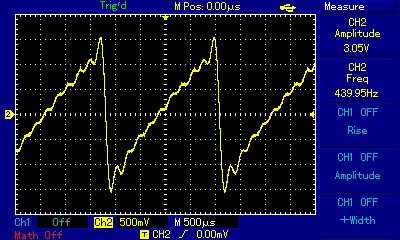
\includegraphics[width=\textwidth]{MAP002.jpg}
  \caption{Sägezahnspannung, bei Synthese bis zur zehnten Oberwelle.}
  \label{fig:Säge}
\end{figure}
\begin{figure}
  \centering
  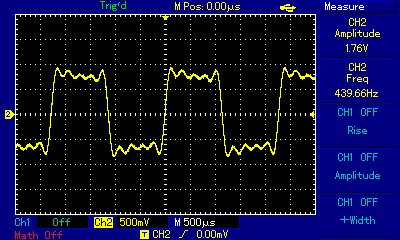
\includegraphics[width=\textwidth]{MAP001.jpg}
  \caption{Rechteckspannung, bei Synthese bis zur zehnten Oberwelle.}
  \label{fig:Recht}
\end{figure}
\begin{figure}
  \centering
  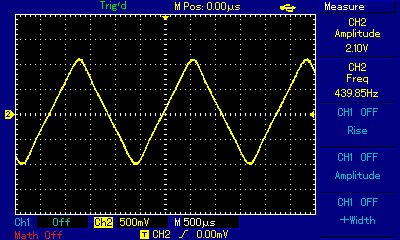
\includegraphics[width=\textwidth]{MAP003.jpg}
  \caption{Dreieckspannung, bei Synthese bis zur zehnten Oberwelle.}
  \label{fig:Drei}
\end{figure}
\clearpage
\section{Diskussion}
Insgesamt sind die Ergebnisse relativ gut. Die bei der Trafo bestimmten Koeffizienten,
der Sägezahnspannung, nehmen genau, wie zuvor berechnet, mit $\frac{1}{n}$ ab.
Die Faktoren, der anderen beiden Spannungsverläufe, zeigen stärkere Abweichungen,
welche auf Schwankungen bei den Amplituden, die am Oszilloskop vermessen wurden,
zurückzuführen sind. Dennoch liegen die Ergebnisse recht nah am Soll.

Bei der Synthese gab es keine größeren Problem die Oberwellen passend einzustellen.
Die Ergebnisse zeigen bereits erkennbar die gewollten Spannungsverläufe. Für einen
genaueren Verlauf würden weitere Oberwellen benötigt.
\nocite{*}
\printbibliography

\end{document}
